\section{Drag and drop}\label{drag-and-drop}

\subsection{What's drag and drop?}\label{whats-drag-and-drop}

Drag and drop is also written as ``Drag-and-Drop'', or ``DND'' in short.
DND is like ``copy and paste'' or ``cut and paste''. If a user drags a
UI element, which is a widget, selected part or something, data is
transferred from the source to the destination.

You probably have experience that you moved a file with DND.

\begin{figure}
\centering
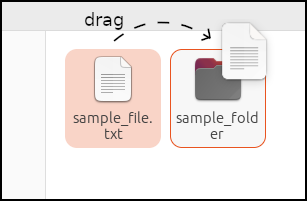
\includegraphics[width=4.6cm,height=3cm]{../image/dnd.png}
\caption{DND on the GUI file manager}
\end{figure}

When the DND starts, the file \passthrough{\lstinline!sample\_file.txt!}
is given to the system. When the DND ends, the system gives
\passthrough{\lstinline!sample\_file.txt!} to the directory
\passthrough{\lstinline!sample\_folder!} in the file manager. Therefore,
it is like ``cut and paste''. The actual behavior may be different from
the explanation here, but the concept is similar.

\subsection{Example for DND}\label{example-for-dnd}

This tutorial provides a simple example in the
\passthrough{\lstinline!src/dnd!} directory. It has three labels for the
source and one label for the destination. The source labels have
``red'', ``green'' or ``blue'' labels. If a user drags the label to the
destination label, the font color will be changed.

\begin{figure}
\centering
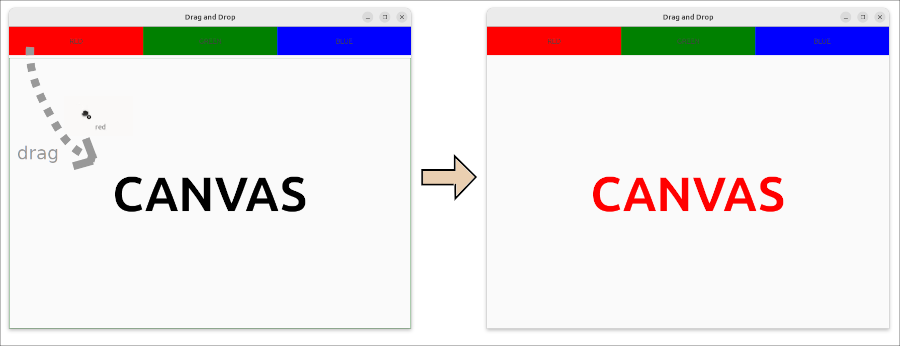
\includegraphics[width=13.5cm,height=5.2cm]{../image/dnd_canvas.png}
\caption{DND example}
\end{figure}

\subsection{UI file}\label{ui-file}

The widgets are defined in the XML file
\passthrough{\lstinline!dnd.ui!}.

\begin{lstlisting}[language=XML, numbers=left]
<?xml version="1.0" encoding="UTF-8"?>
<interface>
  <object class="GtkApplicationWindow" id="win">
    <property name="default-width">800</property>
    <property name="default-height">600</property>
    <property name="resizable">FALSE</property>
    <property name="title">Drag and Drop</property>
    <child>
      <object class="GtkBox">
        <property name="hexpand">TRUE</property>
        <property name="vexpand">TRUE</property>
        <property name="orientation">GTK_ORIENTATION_VERTICAL</property>
        <property name="spacing">5</property>
        <child>
          <object class="GtkBox">
            <property name="orientation">GTK_ORIENTATION_HORIZONTAL</property>
            <property name="homogeneous">TRUE</property>
            <child>
              <object class="GtkLabel" id="red">
                <property name="label">RED</property>
                <property name="justify">GTK_JUSTIFY_CENTER</property>
                <property name="name">red</property>
              </object>
            </child>
            <child>
              <object class="GtkLabel" id="green">
                <property name="label">GREEN</property>
                <property name="justify">GTK_JUSTIFY_CENTER</property>
                <property name="name">green</property>
              </object>
            </child>
            <child>
              <object class="GtkLabel" id="blue">
                <property name="label">BLUE</property>
                <property name="justify">GTK_JUSTIFY_CENTER</property>
                <property name="name">blue</property>
              </object>
            </child>
          </object>
        </child>
        <child>
          <object class="GtkLabel" id="canvas">
            <property name="label">CANVAS</property>
            <property name="justify">GTK_JUSTIFY_CENTER</property>
            <property name="name">canvas</property>
            <property name="hexpand">TRUE</property>
            <property name="vexpand">TRUE</property>
          </object>
        </child>
      </object>
    </child>
  </object>
</interface>
\end{lstlisting}

It is converted to a resource file by
\passthrough{\lstinline!glib-compile-resources!}. The compiler uses an
XML file \passthrough{\lstinline!dnd.gresource.xml!}.

\begin{lstlisting}[language=XML, numbers=left]
<?xml version="1.0" encoding="UTF-8"?>
<gresources>
  <gresource prefix="/com/github/ToshioCP/dnd">
    <file>dnd.ui</file>
  </gresource>
</gresources>
\end{lstlisting}

\subsection{C file dnd.c}\label{c-file-dnd.c}

The C file \passthrough{\lstinline!dnd.c!} isn't a big file. The number
of the lines is less than a hundred. A GtkApplication object is created
in the function \passthrough{\lstinline!main!}.

\begin{lstlisting}[language=C, numbers=left]
int
main (int argc, char **argv) {
  GtkApplication *app;
  int stat;

  app = gtk_application_new (APPLICATION_ID, G_APPLICATION_DEFAULT_FLAGS);
  g_signal_connect (app, "startup", G_CALLBACK (app_startup), NULL);
  g_signal_connect (app, "activate", G_CALLBACK (app_activate), NULL);
  stat =g_application_run (G_APPLICATION (app), argc, argv);
  g_object_unref (app);
  return stat;
}
\end{lstlisting}

The application ID is defined as:

\begin{lstlisting}[language=C]
#define APPLICATION_ID "com.github.ToshioCP.dnd"
\end{lstlisting}

\subsubsection{Startup signal handler}\label{startup-signal-handler}

Most of the work is done in the ``startup'' signal handler.

Two objects GtkDragSource and GtkDropTarget is used for DND
implementation.

\begin{itemize}
\tightlist
\item
  Drag source: A drag source (GtkDragSource instance) is an event
  controller. It initiates a DND operation when the user clicks and
  drags the widget. If a data, in the form of GdkContentProvider, is set
  in advance, it gives the data to the system at the beginning of the
  drag.
\item
  Drop target: A drop target (GtkDropTarget) is also an event
  controller. You can get the data in the GtkDropTarget::drop signal
  handler.
\end{itemize}

The example below uses these objects in a very simple way. You can use
number of features that the two objects have. See the following links
for more information.

\begin{itemize}
\tightlist
\item
  \href{https://docs.gtk.org/gtk4/drag-and-drop.html}{Drag-and-Drop in
  GTK}
\item
  \href{https://docs.gtk.org/gtk4/class.DragSource.html}{GtkDragSource}
\item
  \href{https://docs.gtk.org/gtk4/class.DropTarget.html}{GtkDropTarget}
\end{itemize}

\begin{lstlisting}[language=C, numbers=left]
static void
app_startup (GApplication *application) {
  GtkApplication *app = GTK_APPLICATION (application);
  GtkBuilder *build;
  GtkWindow *win;
  GtkLabel *src_labels[3];
  int i;
  GtkLabel *canvas;
  GtkDragSource *src;
  GdkContentProvider* content;
  GtkDropTarget *tgt;
  GdkDisplay *display;
  char *s;

  build = gtk_builder_new_from_resource ("/com/github/ToshioCP/dnd/dnd.ui");
  win = GTK_WINDOW (gtk_builder_get_object (build, "win"));
  src_labels[0] = GTK_LABEL (gtk_builder_get_object (build, "red"));
  src_labels[1] = GTK_LABEL (gtk_builder_get_object (build, "green"));
  src_labels[2] = GTK_LABEL (gtk_builder_get_object (build, "blue"));
  canvas = GTK_LABEL (gtk_builder_get_object (build, "canvas"));
  gtk_window_set_application (win, app);
  g_object_unref (build);

  for (i=0; i<3; ++i) {
    src = gtk_drag_source_new ();
    content = gdk_content_provider_new_typed (G_TYPE_STRING, gtk_widget_get_name (GTK_WIDGET (src_labels[i])));
    gtk_drag_source_set_content (src, content);
    g_object_unref (content);
    gtk_widget_add_controller (GTK_WIDGET (src_labels[i]), GTK_EVENT_CONTROLLER (src)); // The ownership of src is taken by the instance.
  }

  tgt = gtk_drop_target_new (G_TYPE_STRING, GDK_ACTION_COPY);
  g_signal_connect (tgt, "drop", G_CALLBACK (drop_cb), NULL);
  gtk_widget_add_controller (GTK_WIDGET (canvas), GTK_EVENT_CONTROLLER (tgt)); // The ownership of tgt is taken by the instance.

  provider = gtk_css_provider_new ();
  s = g_strdup_printf (format, "black");
  gtk_css_provider_load_from_data (provider, s, -1);
  g_free (s);
  display = gdk_display_get_default ();
  gtk_style_context_add_provider_for_display (display, GTK_STYLE_PROVIDER (provider),
                                              GTK_STYLE_PROVIDER_PRIORITY_APPLICATION);
  g_object_unref (provider); // The provider is still alive because the display owns it.
}
\end{lstlisting}

\begin{itemize}
\tightlist
\item
  15-22: Builds the widgets. The array
  \passthrough{\lstinline!source\_labels[]!} points the source labels
  red, green and blue in the ui file. The variable
  \passthrough{\lstinline!canvas!} points the destination label.
\item
  24-30: Sets the DND source widgets. The for-loop carries out through
  the array \passthrough{\lstinline!src\_labels[]!} each of which points
  the source widget, red, green or blue label.
\item
  25: Creates a new GtkDragSource instance.
\item
  26: Creates a new GdkContentProvider instance with the string ``red'',
  ``green'' or ``blue. They are the name of the widgets. These strings
  are the data to transfer through the DND operation.
\item
  27: Sets the content of the drag source to the GdkContentProvider
  instance above.
\item
  28: Content is useless so it is destroyed.
\item
  29: Add the event controller, which is actually the drag source, to
  the widget. If a DND operation starts on the widget, the corresponding
  drag source works and the data is given to the system.
\item
  32-34: Sets the DND drop target.
\item
  32: Creates a new GtkDropTarget instance. The first parameter is the
  GType of the data. The second parameter is a GdkDragAction enumerate
  constant. The arguments here are string type and the constant for
  copy.
\item
  33: Connects the ``drop'' signal and the handler
  \passthrough{\lstinline!drop\_cb!}.
\item
  34: Add the event controller, which is actually the drop target, to
  the widget.
\item
  36-43: Sets CSS.
\item
  37: A varable \passthrough{\lstinline!format!} is static and defined
  at the top of the program. Static variables are shown below.
\end{itemize}

\begin{lstlisting}[language=C]
static GtkCssProvider *provider = NULL;
static const char *format = "label {padding: 20px;} label#red {background: red;} "
  "label#green {background: green;} label#blue {background: blue;} "
  "label#canvas {color: %s; font-weight: bold; font-size: 72pt;}";
\end{lstlisting}

\subsubsection{Activate signal handler}\label{activate-signal-handler}

\begin{lstlisting}[language=C, numbers=left]
static void
app_activate (GApplication *application) {
  GtkApplication *app = GTK_APPLICATION (application);
  GtkWindow *win;

  win = gtk_application_get_active_window (app);
  gtk_window_present (win);
}
\end{lstlisting}

This handler just shows the window.

\subsubsection{Drop signal handler}\label{drop-signal-handler}

\begin{lstlisting}[language=C, numbers=left]
static gboolean
drop_cb (GtkDropTarget* self, const GValue* value, gdouble x, gdouble y, gpointer user_data) {
  char *s;

  s = g_strdup_printf (format, g_value_get_string (value));
  gtk_css_provider_load_from_data (provider, s, -1);
  g_free (s);
  return TRUE;
}
\end{lstlisting}

The ``drop'' signal handler has five parameters.

\begin{itemize}
\tightlist
\item
  GtkDropTarget instance on which the signal has been emitted.
\item
  GValue that holds the data from the source.
\item
  The arguments \passthrough{\lstinline!x!} and
  \passthrough{\lstinline!y!} are the coordinate of the mouse when
  released.
\item
  User data was set when the signal and handler was connected.
\end{itemize}

The string from the GValue is ``red'', ``green'' or ``blue''. It
replaces ``\%s'' in the variable \passthrough{\lstinline!format!}. That
means the font color of the label \passthrough{\lstinline!canvas!} will
turn to the color.

\subsection{Meson.build}\label{meson.build}

The file \passthrough{\lstinline!meson.build!} controls the building
process.

\begin{lstlisting}[numbers=left]
project('dnd', 'c')

gtkdep = dependency('gtk4')

gnome = import('gnome')
resources = gnome.compile_resources('resources','dnd.gresource.xml')

executable(meson.project_name(), 'dnd.c', resources, dependencies: gtkdep, export_dynamic: true, install: false)
\end{lstlisting}

You can build it from the command line.

\begin{lstlisting}
$ cd src/dnd
$ meson setup _build
$ ninja -C _build
$ _build/dnd
\end{lstlisting}

The source files are under the directory
\passthrough{\lstinline!src/dnd!} of the
\href{https://github.com/ToshioCP/Gtk4-tutorial}{repository}. Download
it and see the directory.
